\documentclass[tikz,border=3pt]{standalone}
\usetikzlibrary{arrows.meta,decorations.pathmorphing}
\begin{document}
\pgfmathsetseed{31415}
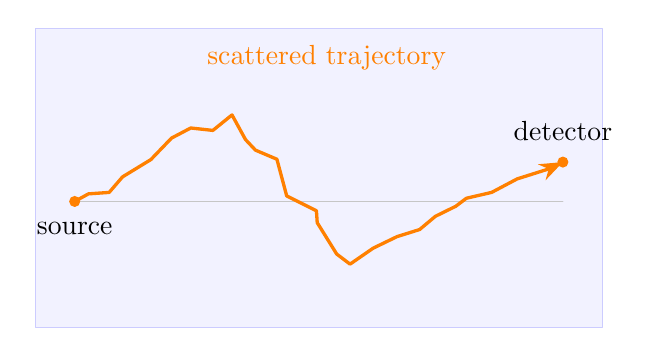
\begin{tikzpicture}[x=1cm,y=1cm,>=Stealth,line cap=round,line join=round]
  \draw[fill=blue!5,draw=blue!20] (-.5,-1.6) rectangle (6.7,2.2);
  \draw[gray!45] (0,0) -- (6.2,0);
  \draw[orange,very thick,-Stealth,decorate,
    decoration={random steps,segment length=3mm,amplitude=1.2mm,pre length=2mm,post length=2mm}]
    (0,0) -- (2,1.1) -- (3.5,-.8) -- (6.2,.5);
  \fill[orange] (0,0) circle (2pt);
  \fill[orange] (6.2,.5) circle (2pt);
  \node[below] at (0,-.15) {source};
  \node[above] at (6.2,.65) {detector};
  \node[orange,above] at (3.2,1.55) {scattered trajectory};
\end{tikzpicture}
\end{document}
